%This is chapter 3
%%=========================================
\chapter[Method]{Materials and methods}

%In this final chapter you should sum up what you have done and which results you have got. You should also discuss your findings, and give recommendations for further work.

%%=========================================

\section{Tools and libraries}
\subsection{JavaScript}
JavaScript has mainly been chosen as the base implementation language because of its cross compatibility and popularity. ...

\subsection{Babel}
- Babel - ES6 needs to be transpiled to ES5 (Browser compatibility).
\subsection{npm}
Needed packages.. Published all packages to npm.. Most stabile compared to GitHubs new repo....

\subsection{Third party libraries}
Why did i use them???
list up like:
- xxx because ...
- xxx provides ...
Elaborate some on three.js - why is it good? (popularity)

\subsection{GitHub Actions}
Why? How did i use it? - For automation... - deeply integrated in GitHub.

\section{Working methodology}
\subsection{Scrum}
Even though this is a one man project, i have tried to adapt the scrum methodology.
...

\subsection{Requirements specification}
\subsubsection{Acceptance criteria}
Acceptance criteria - custom field in Jira.
Specially for the voxelization algorithm?

\subsection{GitFlow}
Why did i follow gitflow? Any changes to the usage?? Good for enforcing standards, automation etc..

\subsection{Semantic versioning}
All published modules are enforcing Semantic versioning. This ....

\section{three-voxel-loader}
\colorbox{green}{NEED UML DIAGRAMS}\\
The main goal for the three-voxel-loader is to generate a 3D mesh based on voxel data. The next subsections will present a walkthrough of how the plugin is implemented, including the various design choices made.

\subsection{Internal data structure}
For the plugin to be able support loading of various voxel data formats, an internal data structure is used. This serves as an interface for the processing of various voxel data internally in the plugin. The chosen data structure is an octree, as described in Section~\ref{sec:theory-octree}. There are several reasons behind this choice. 

Voxel data normally consists of very large amounts of data. One of the main limitations for how big a dataset can be, is the amount of available computer memory (RAM). The memory footprint of the plugin is therefore a big concern, especially since the targeted runtime environments are often placing further restrictions on the available memory resources. Voxel data normally contains very large amounts of empty space, or "air". This data is not needed for generating the polygon mesh. Only the data about the actual voxels and their locations are of interest. The location of the voxels are normally not stored explicitly, but rather derived by their relative location to neighboring voxel cells. An octree is especially well suited for this purpose. Since an octree is based on partitioning of space, large amounts of this empty space in the voxel data can be discarded. This works especially well if the voxel data is clustered.

Octrees also makes it easy to implement a Level of Detail (LOD) mechanism. By determining the desired depth of the octree, one are able to simplify the detail of the voxel data. This is very valuable, as generating mesh geometry for every voxel is placing high stress on the available hardware resources. Being able to control the LOD, this can be very effective in terms of simplifying the resulting mesh.

\subsection{Loading voxel data}
In order to actually load the voxel data (by generating an octree), several loader classes have been created. These classes all extend the \textit{loader} class defined in three.js, providing both consistency and tight integration with library. It also ensures that extending the support for more file loaders in the future is easy. Finally, a factory pattern has been implemented for getting and instantiating the desired voxel loader. This makes it able to define an easy-to-use API, where the user only needs to supply the actual voxel data and the corresponding format.

The currently implemented loaders supports several file formats, including XML, VOX and BINVOX. It is also possible to import plain 3D arrays. Following is a brief description of these loaders.
\begin{itemize}
    \item \textbf{XML} - XML is an incredible versatile file format. For implementing the XML loading, the native JavaScript DOM parser is used for the actual parsing of the XML data. The required format of the XML document structure is described on the GitHub wiki page for the plugin. \colorbox{red}{PROVIDE LINK HERE!!!!!}
    \item \textbf{VOX} - VOX files are loaded with a third party package named \textit{format-vox}~\cite{format-vox}. The VOX file format is provided by MagicaVoxel, a popular voxel graphics editor.
    \item \textbf{BINVOX} - BINVOX \cite{binvox-file-format} is one of the more popular voxel data file formats. BINVOX is the file format used by the binvox~\cite{binvox} voxelization software. A separate repository~\cite{andstor-binvox} named has been created for handling BINVOX files. See Section \ref{sec:method-binvox}
    \item \textbf{3D array} - The 3D array loader is implemented by simply iterating the multidimensional array.
\end{itemize}

\subsection{Visualization}
The most intuitive way to visualize a voxel is in the form of a cube. BoxBufferGeometry from three.js has therefore been used to generate the individual 3D visualization of the voxels. However, one BoxBuffer geometry consists of no less than twelve triangles. The number of triangles generated for visualizing the mesh is therefore twelve times the number of voxels. One of the more time consuming operations in terms of actually displaying the 3D graphics, is the number of draw calls made to the graphics API. In order to limit this, all the generated box meshes are merged into one big mesh.

\subsection{Debugging}
For actually developing and testing the plugin, a HTML page was created. The page includes basic setup of three.js, alongside various input controls for inspecting and testing the three-voxel-loader plugin. The input controls are provided by a lightweight JavaScript controller library named dat.gui~\cite{dat.gui}. In the end, the debugging solution were polished and deployed to GitHub Pages, serving as an example for the various functionality the plugin provides. \colorbox{red}{LINK TO GITHUB PAGES EXAMPLE}

\section{Voxelizer}
Short intro
Three.js provides raycasting out  of the box. However, the raycasting method implemented It would be more efficient to implement the raycasting directly without the use of three.js. However, this would be laboursome. However, the main reason for using the three.js library is based on the popularity of the project. the ecosystem of three.js is vast, providing everything from file loaders to ... This, combined with excellent documentation, should make it very easy to produce a 3D model in three.js. This sets the stage for further processing of the 3D models with the Voxelizer engine.

\subsection{implementation}
\colorbox{RubineRed}{UML diagram of system here}

The system is broken down in several modules (folders). This includes:
\begin{itemize}
    \item \textbf{core} - The core module contains core APIs. This provides the main user API for conducting the voxelization.
    \item \textbf{algorithms} - The algorithm module defines the algorithm system. This is in charge for the actual sampling of the 3D models.
    \item \textbf{color} - The coloring system is found in the color module. This manages the color extraction for supporting color voxelization.
    \item \textbf{volume} - The volume module mainly contains a wrapper class for providing a consistent interface for interacting with volumes throughout the application.  
    \item \textbf{exporters} - The exporters module is made up of various exporter classes. These provides 
    \item \textbf{utils} - This module contains various utility functions.
\end{itemize}

\subsection{Algorithm system}
Voxelizer implements an algorithm system that makes it easy to extend the voxelization support. Be it new algorithm types or options. The system mainly consists of two base abstract algorithm classes. One for plain voxelization, and one which is colorable. By simply extending the appropriate base class, a new algorithm can be defined. Further, a factory pattern has been implemented for selecting the appropriate algorithm.

Since the generated voxel data can be huge, an efficient internal data structure needs to be used. Here is two main concerns to take into account. The first is the memory footprint. In order to be able to do high resolution voxelizations, a limiting factor is the amount of available system memory. A second and bigger concern is speed. The JavaScript engines are able to do quite a lot of optimization. By using the JavaScript language in clever ways, quite high processing speeds can be achieved.

The old Voxelizer v0.1.3 used normal JavaScript arrays which was nested. These arrays grows and shrink dynamically, potentially resulting in slow performance. Although, the JavaScript engines are often able to optimize the execution quite a bit, resulting in decent speeds. However, in order to comply with both the memory and performance requirements, typed arrays have been used instead. More specifically, only one large one-dimensional typed array is used. This is a more low level data type than normal arrays, providing mechanism for reading and writing raw binary data in memory buffers. In order to support multidimensionality, the efficient third party library ndarray is used. See Section \ref{sec:theory-ndarray} for more details on ndarray.

\subsection{Raycasting algorithm}
\label{sec:method-raycasting-algorithm}
The new and upgraded voxelization algorithm is mainly based on raycasting (see Section \ref{sec:theory-raycasting}). Following is a description of how the algorithm works.

First, several preparations are made on the mesh. Firstly, the mesh is centered at the origin. Then the mesh is manipulated to include both front and back faces. This ensures that raycasting against the mesh will result in a hit against both front and back sides of the model. This means that it is not needed to raycast from all 6 sides of the mesh. Hence, the algorithm samples the mesh from the front, left and top sides. These results are then merged together, and returned to the user in form of an ndarray. Figure \ref{fig:voxel-sample-merging} illustrates how these three results are merged, resulting in a complete surface representation.
\begin{figure}[h]
    \centering
    \begin{subfigure}[t]{0.3\textwidth}
        \centering
        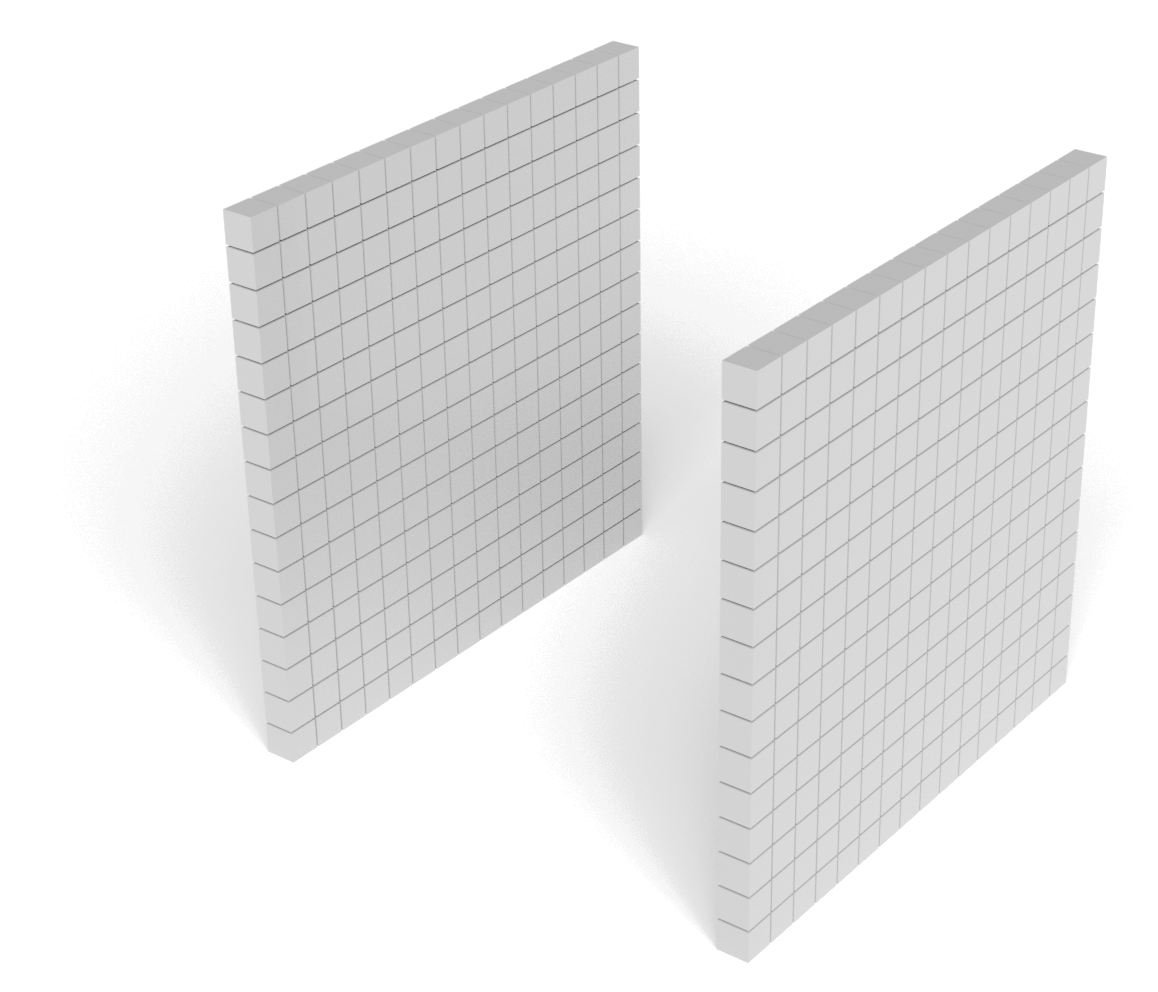
\includegraphics[width=\textwidth]{sections/methodology/figures/voxels-merge-1.png}
        \caption{Front side sample.}
        \label{fig:filling-non-watertight-model}
    \end{subfigure}
    \hfill
    \begin{subfigure}[t]{0.3\textwidth}
        \centering
        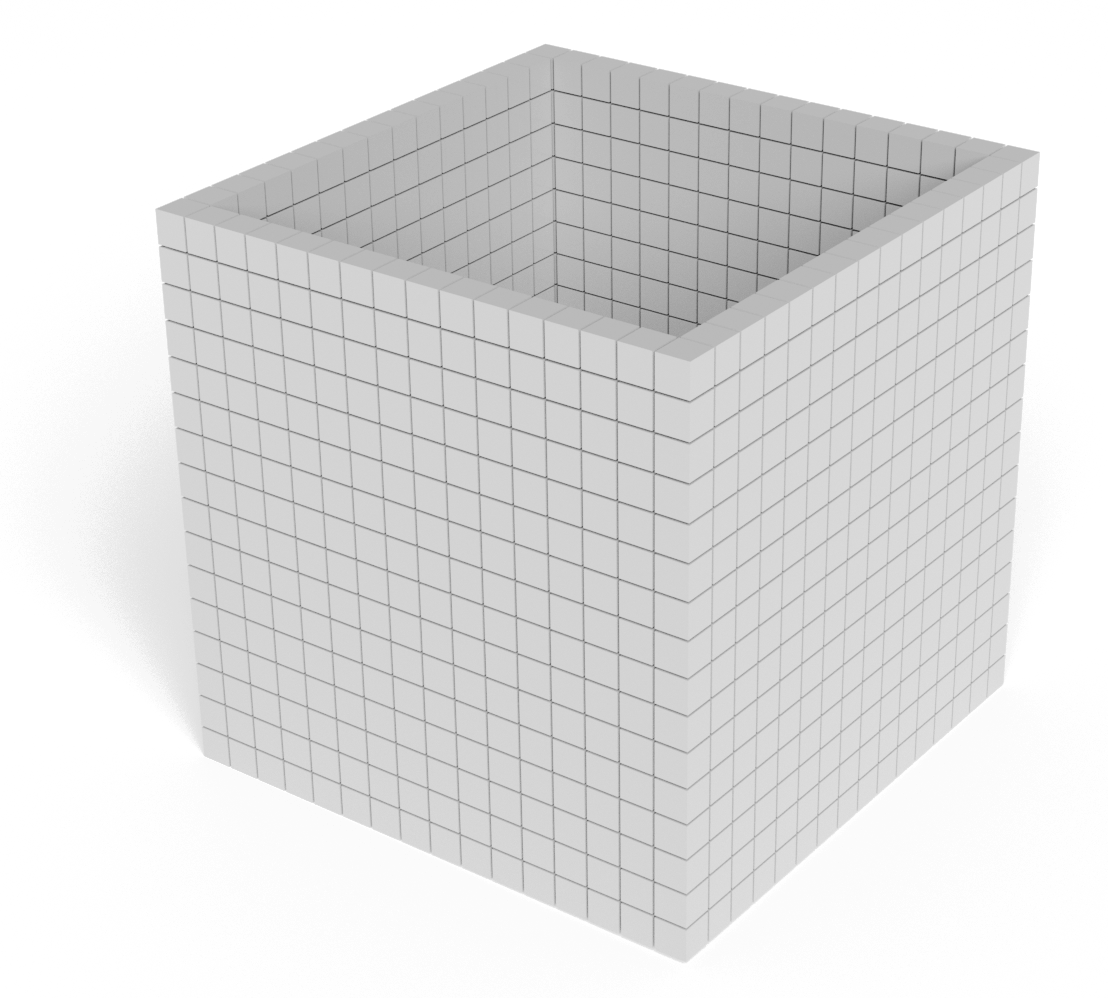
\includegraphics[width=\textwidth]{sections/methodology/figures/voxels-merge-2.png}
        \caption{Front and left side samples merged together.}
        \label{fig:filling-watertight-model}
    \end{subfigure}
    \hfill
    \begin{subfigure}[t]{0.3\textwidth}
        \centering
        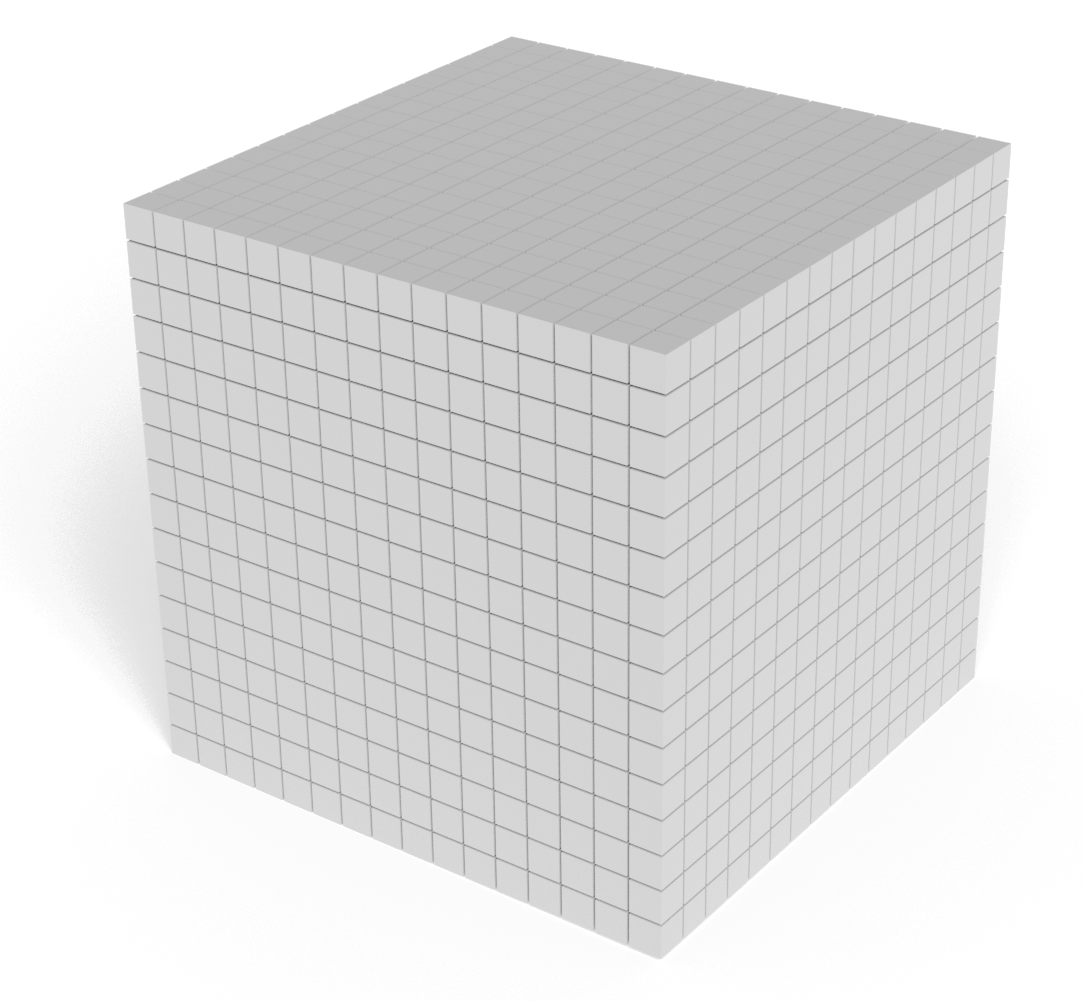
\includegraphics[width=\textwidth]{sections/methodology/figures/voxels-merge-3.png}
        \caption{Front, left and top side samples merged together.}
        \label{fig:filling-watertight-model}
    \end{subfigure}
       \caption{Merging of voxel samplings.}
       \label{fig:voxel-sample-merging}
\end{figure}

\subsection{three.js optimization}
The raycasting functionality, used by the raycasting algorithm described in Section \ref{sec:method-raycasting-algorithm}, is supplied by the three.js library. The library provides a throughly tested and accurate raycasting solution. However, it is CPU bound and  iterates every face of the mesh. This gives each raycasting operation a time complexity of O(n). If the 3D mesh is highly detailed, containing a large amount of polygons, the raycasting will take a long time to perform. After a careful assessment of potential solutions, the three.js plugin named three-bvh-mesh \cite{three-bvh-mesh} was used to improve this. This plugin provides a BVH implementation in order to speed up the raycasting against three.js meshes. By using this plugin, the time complexity for a single raycasting operation decreases from O(n) to O(log~n). Figure \ref{fig:bvh-monkey} shows an example visualization of a BVH tree applied to a 3D model, which is generated by the three-bvh-mesh plugin.

\begin{figure}[ht]
    \centering
    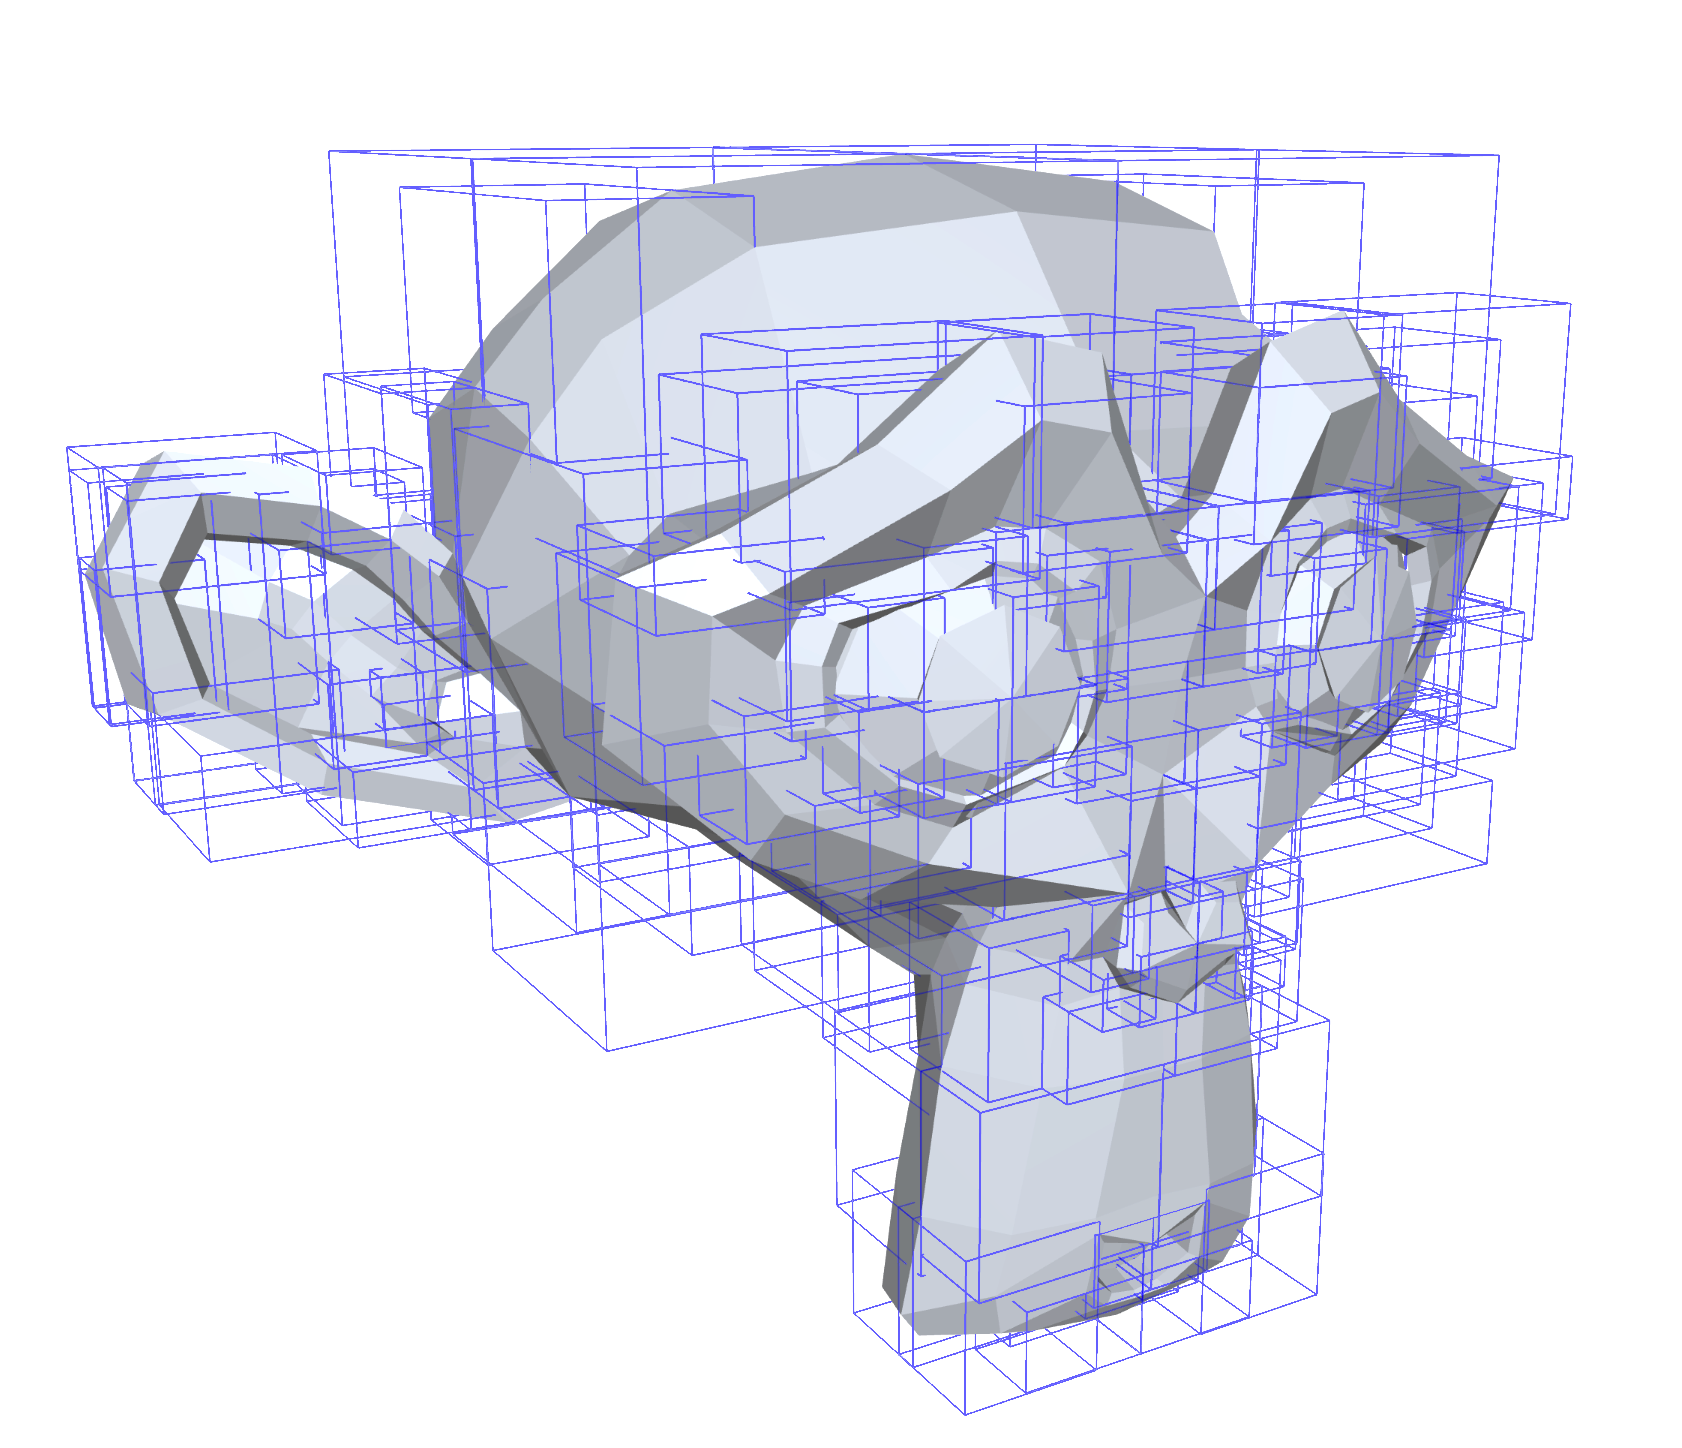
\includegraphics[width=0.5\textwidth]{sections/methodology/figures/bvh-monkey.png}
    \caption{Visualization of BVH applied to 3D model.}
    \label{fig:bvh-monkey}
\end{figure}

\subsubsection{Shell voxelization}
Asd

\subsubsection{Solid voxelization}
\colorbox{RubineRed}{Maybe more discussion or result related?}
The solid voxelisation, or filled voxelisation, is achieved by interpreting the first raycast intersect as the surface of the object. From this point will everything be considered "inside" the object. When a second intersect is detected, the state is changed to be "outside" the object. A new hit would indicate "inside", and so on. This works verry well with a watertight (\colorbox{RubineRed}{edges are manifolded?}) 3D model, as can be seen from figure \ref{fig:filling-non-watertight-model}. However, when trying to fill an object which is not watertight, this can result in severe inaccuracies. This can be seen in figure \ref{fig:filling-watertight-model}

\begin{figure}[h]
    \centering
    \begin{subfigure}[b]{0.45\textwidth}
        \centering
        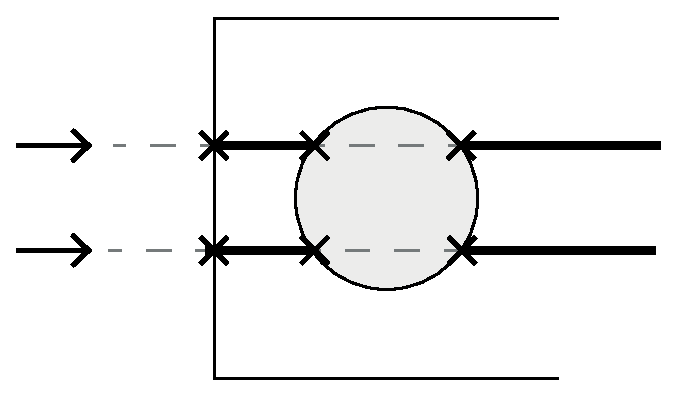
\includegraphics[width=\textwidth]{sections/methodology/figures/solid-non-watertight}
        \caption{Non-watertight 3D model cross section.}
        \label{fig:filling-non-watertight-model}
    \end{subfigure}
    \hfill
    \begin{subfigure}[b]{0.45\textwidth}
        \centering
        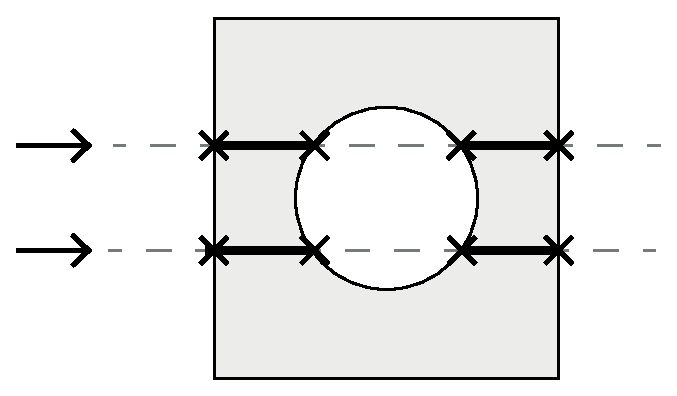
\includegraphics[width=\textwidth]{sections/methodology/figures/solid-watertight}
        \caption{Watertight 3D model cross section.}
        \label{fig:filling-watertight-model}
    \end{subfigure}
       \caption{Solid (voxelization) filling of 3D model cross section.}
       \label{fig:filling-3d-model}
\end{figure}


\subsection{Color system}
Reads object texture maps, extracts color etc...

\subsection{Loading}
The Voxelizer library/engine previously made use of a wrapper OBJ loader.
This support has been dropped in favor of the ES6 JS modules provided by three.js.

\subsection{Exporting}
- XML
- BINVOX (Separate repo)
- 3D array

\subsection{Testing}
Several unit tests are created for testing the different parts of the voxelization system. This ensures correct operation of the voxelization process, and protect against introducing new bugs.  Jest has been chosen as the testing framework provider. The 
\subsection{Migration}


\subsection{Debugging}
Developed an example -> later polished so you can find it on github...

\section{BINVOX}
\label{sec:method-binvox}
A separate repo for building and parsing binvox files were constructed during refactoring of the voxelizer and the three-voxel-loader plugin....
\lstinputlisting[language=JSON,style=numbers,caption={Example BINVOX data in JSON format}]{sections/methodology/code/binvox-json.json}


\section{Voxelizer-Desktop}
\subsection{Electron}
\subsubsection{Auto updating}

\subsection{GUI}
... Sketches?? Wireframe diagrams of GUI etc...


\section{JSDoc Action}
Implementation in JS, not docker. Gives best possible speed, and cross compatibility (Win, linux and macos)
Can be used with any other action to upload to the desired service, for example GitHub pages.

\colorbox{RubineRed}{Diagram of implementation here}

\subsection{JSDoc}
Passes to cmd, loads configs, etc....

\subsection{Templates}
Support for templates. Downloads with the help of npm. Can be a github repository, npm package, etc...

\section{Automation}
\subsection{Workflows}
GitHub Actions...
Figure \ref{fig:cicd-pipelines} shows the continous integration and continous development pipelines. Describe how they work here....
\begin{figure}[h]
    \setlength{\abovecaptionskip}{25pt}
    \centering
    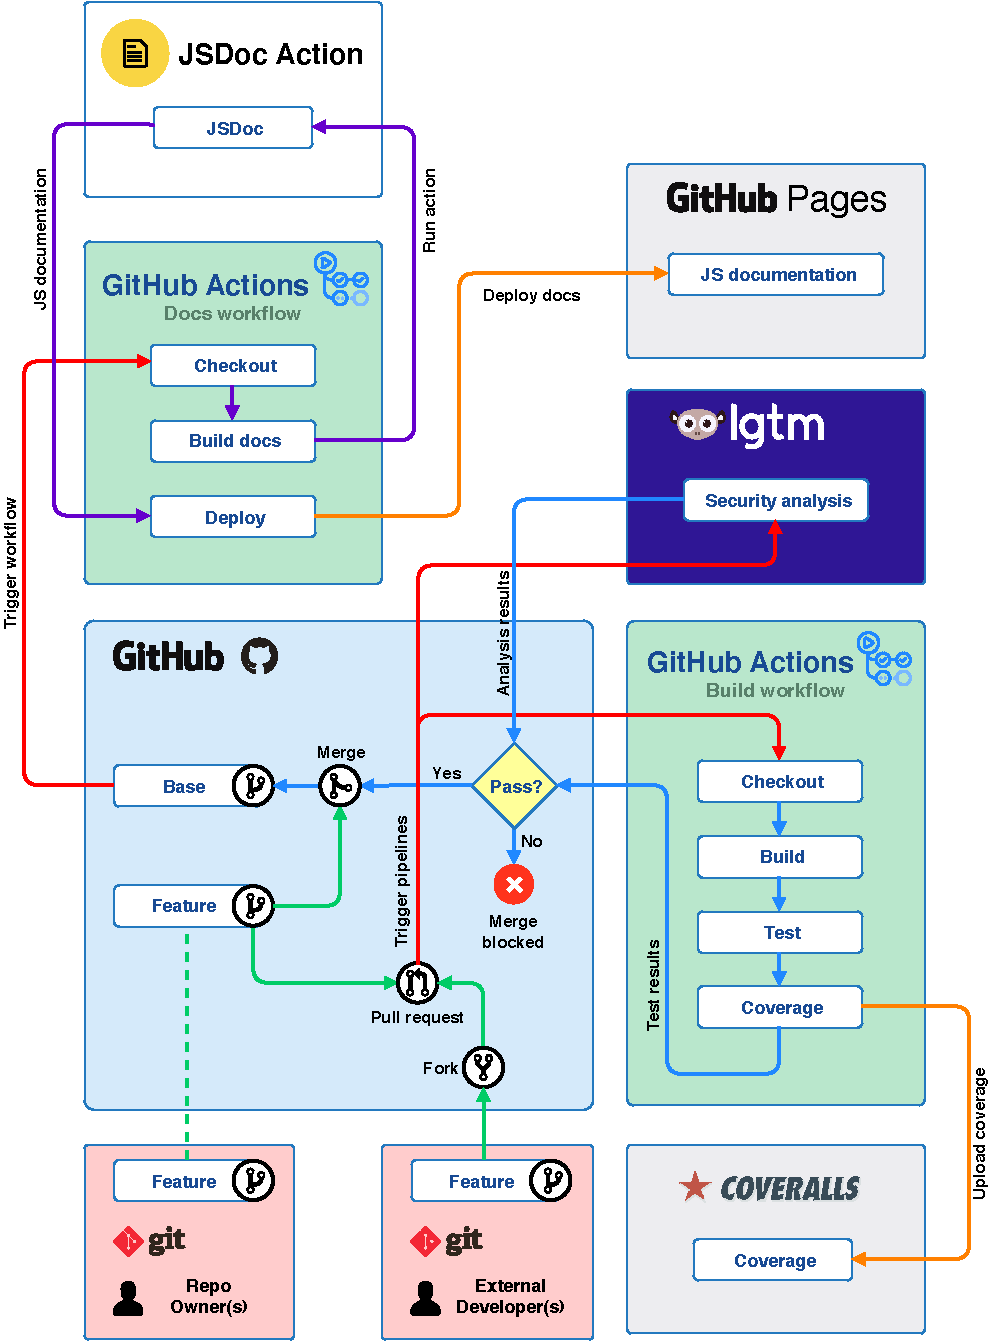
\includegraphics[page=1,scale=1]{sections/methodology/figures/pipelines.pdf}
    \caption{CI/CD pipelines}
    \label{fig:cicd-pipelines}
\end{figure}
\clearpage

And continue explaining here....
\subsubsection{Build}
\subsubsection{Test}
\subsubsection{Coverage}
Coveralls
\subsubsection{Security analysis}
LGTM
\subsubsection{Documentation generation}
JSDoc Action -> GitHub pages

\subsection{Release automation}

\subsubsection{Publish package}
See figure \ref{fig:release-automation}
\begin{figure}[h]
    \setlength{\abovecaptionskip}{25pt}
    \centering
    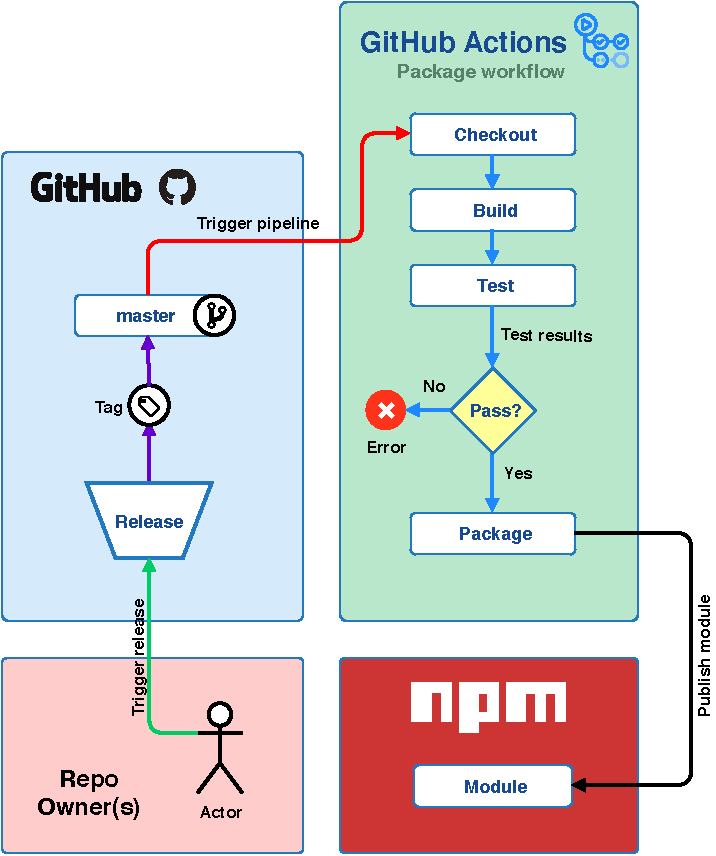
\includegraphics[page=1,scale=1]{sections/methodology/figures/package-release-automation.pdf}
    \caption{Automation of release publishing process.}
    \label{fig:release-automation}
\end{figure}

\subsubsection{GitHub Action version tagging}
Auto major version tagging update
See figure \ref{fig:update-major-tag}

\begin{figure}[h]
    \setlength{\abovecaptionskip}{25pt}
    \centering
    \hspace*{-2cm}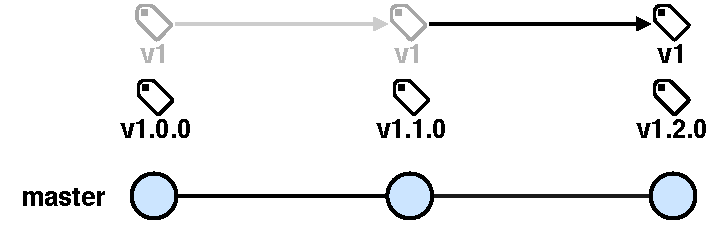
\includegraphics[page=1,scale=1]{sections/methodology/figures/update-major-tag.pdf}
    \caption{Automatic updating of major version tag.}
    \label{fig:update-major-tag}
\end{figure}

\subsection{Dependency updating}
Automated by Dependabot (accuired by GitHub).

\subsection{LaTeX generation}
Include how i have setup automation between my latex projects in order to generate thesis?

\section{file-existence-action}
During development of the workflows, it became apparent that i needed to be able to check if a file existed, and use this result in the following steps of the workflow.  This resulted in a relatively small GitHub action, named File Existence.

\section{file-reader-action}
During development of the workflows, it became apparent that i needed to be able to read the contents of a file, in order to check if it was empty and in that case, terminate the workflow. this resulted in a very small GitHub action, named File Reader.